\section{Introduction}

The new Wi-Fi standard IEEE~802.11ah \cite{80211ahStd}, targeting large scale and low-power \gls{iot} network scenarios, proposes a novel station-grouping based medium access method, referred to as \gls{raw}. In particular, stations are divided into groups, and a group of stations are only allowed to access the channel at a specific time interval, in order to reduce contention and collisions in highly dense deployments. It is a flexible hybrid channel access method, allowing up to 8192 stations connected to a single \gls{ap}, is highly suitable to provide scalable connectivity to both sparsely and densely deployed low-power devices. 


\begin{figure}[t]
  \centering
  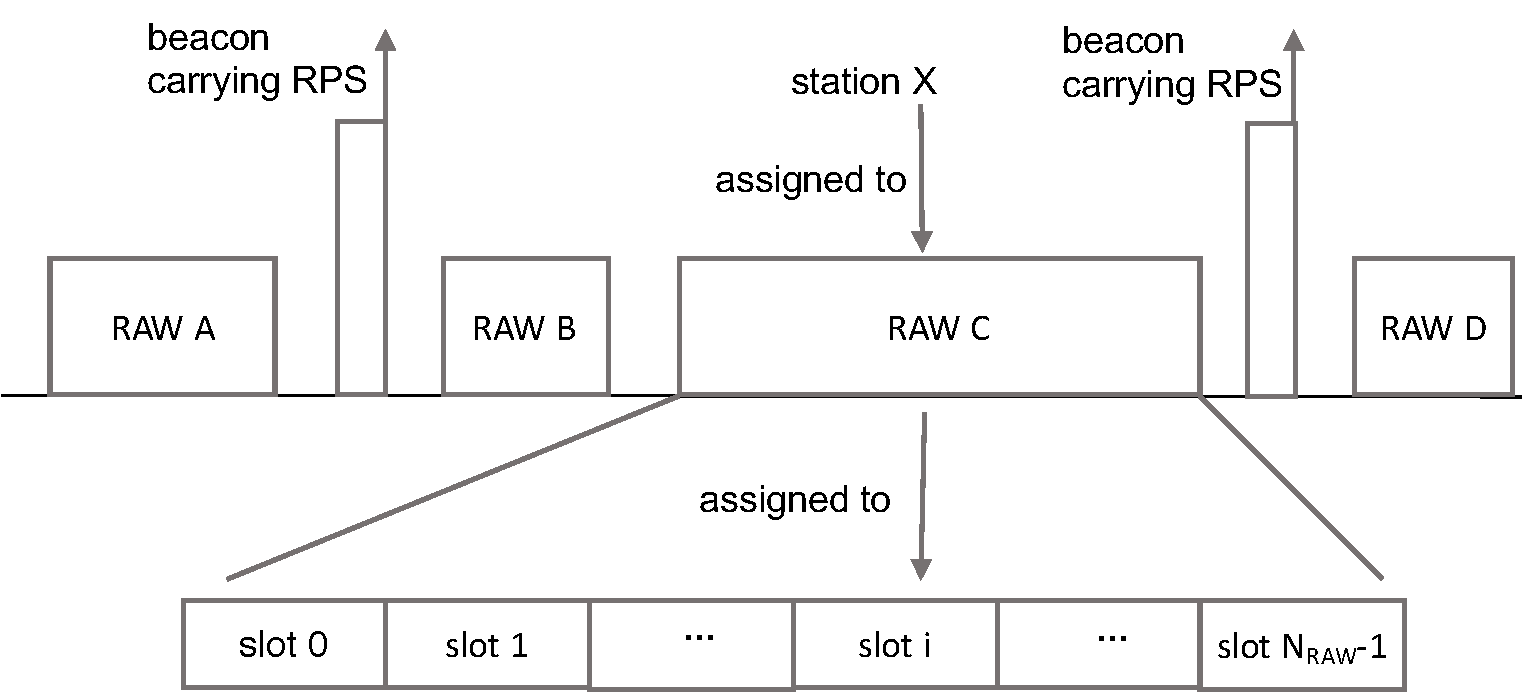
\includegraphics[width=0.8\columnwidth]{figures/raw}
  \caption{Schematic representation of the \gls{raw} mechanism.\label{fig:RAW}}
\end{figure}

%The proposed \gls{raw} feature in 802.11ah aims to reduce collisions and improve performance in dense \gls{iot} network where hundreds or even thousands of stations are simultaneously contending for channel access. It restricts the number of stations that can simultaneously access the channel by splitting them into groups and only allowing stations that belong to a certain group to access the channel at specific times.

Figure \ref{fig:RAW} schematically depicts how RAW works. Specifically, the airtime is split into intervals, some of which are assigned to RAW groups, while the others are considered as shared channel airtime and can be accessed by all stations. 

At fixed intervals a beacon frame is transmitted,
carrying a \gls{rps} information element. The \gls{rps} specifies the stations that belong to the group, as
well as the interval start time.

Moreover, each RAW interval(group) consists of one or more slots, over which the stations in the RAW group are split evenly (using round robin assignment). Therefore, the \gls{raw} related parameters include \textit{ the number of stations assigned to the \gls{raw} groups, number of \gls{raw} groups, duration of each \gls{raw} group}, and  \textit{number of slots in each \gls{raw} group}. For a more in-depth description of \gls{raw} and IEEE~802.11ah, the reader is referred to existing literature~\cite{80211ahStd, Khorov2015a, sensors80211ah}.
 %Sensor2017

% Figure~\ref{fig:RAW} schematically depicts how \gls{raw} works. Specifically, the channel airtime is split into several intervals, some of which are assigned to RAW groups, while others are shared and can be accessed by all stations using the traditional 802.11 \gls{edca}, which rely on \gls{csma} channel access. At fixed intervals a beacon frame is transmitted, carrying a \gls{rps} information element. The \gls{rps} specifies the stations belonging to each group using the start and end \gls{aid}, the group start time, and duration. Moreover, each RAW group consists of one or more equal-duration slots, among which the stations assigned to the RAW group are evenly split (using round robin assignment). The \gls{rps} information element also contains the number of slots, slot format and slot duration count sub-fields, which jointly determine the RAW slot duration. For a more in-depth description of \gls{raw}, the reader is referred to existing literature~\cite{Khorov2015a,Sensor2017}.

% \begin{figure}[t]
%   \centering
%   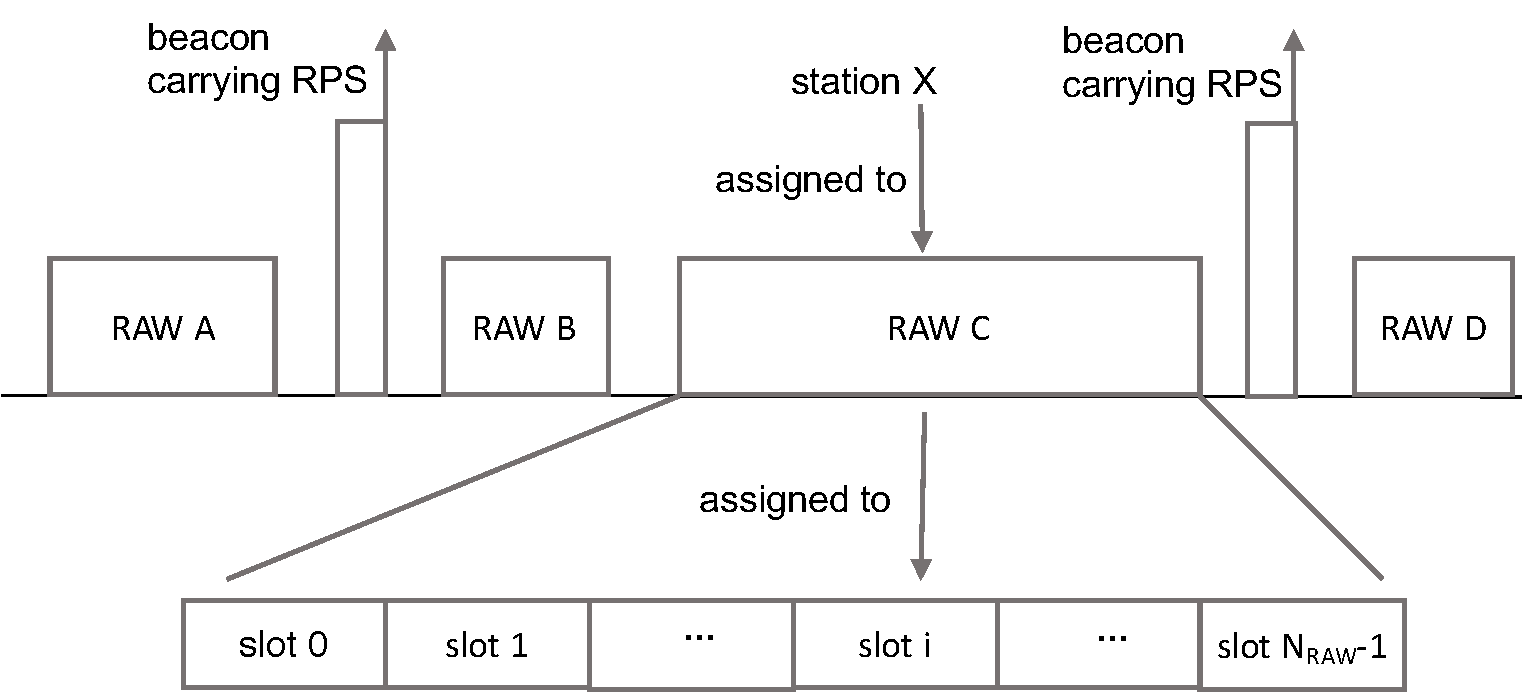
\includegraphics[width=0.8\columnwidth]{figures/raw}
%   \caption{Schematic representation of the \gls{raw} mechanism.\label{fig:RAW}}
% \end{figure}

An extensive evaluation on \gls{raw} has been conducted in ~\cite{WoWMoM2016}. The results demonstrate that, with appropriate \gls{raw} configuration, the \gls{raw} mechanism can provide substantial performance (e.g., throughput, delay and energy consumption) improvement over the legacy channel access method \gls{edca}, in particular for highly-loaded dense network scenarios. One the other hand, the incorrect \gls{raw} configuration severely deteriorates performance. Moreover, it reveals the optimal \gls{raw} parameters are affected by a variety of network-related parameters. For instance, the number of stations, traffic patterns, and network load. Therefore, in order to configure \gls{raw} with the optimal parameters, a model on \gls{raw} is needed to be able to predict the performance for the given \gls{raw} parameter values and given network conditions. Concretely, the model takes network conditions and a \gls{raw} configuration as input, and predicts one or more performance metrics (e.g., throughput or energy consumption) as output. Although several \gls{raw} models have been proposed, they are either too computationally hard to be used in real-time, or rely on certain simplifications (e.g., no capture effect, no hidden nodes, homogeneous stations, saturated traffic). Such simplifications limit the usage of the \gls{raw} models, making it difficult to apply them to realistic \gls{iot} networks.

In this paper, we present a surrogate model that models \gls{raw} performance for realistic \gls{iot} scenarios. The model is trained using realistic simulation results (with capture effect enabled and the presence of hidden nodes), and supports heterogeneous stations with different \gls{mcs} and packet size. Although the \gls{raw} configuration depends on many input variables that leads to a wide range of value, the model can be accurately trained with very few labeled sample data points. Moreover, once trained, evaluating the model is equivalent to a constant-time table lookup, which can be easily executed in real-time. To the best of our knowledge, this is the first \gls{raw} model that support heterogeneous stations with different MCSs and packet sizes.


The remainder of this paper is structured as follows. Section~\ref{sec:related_work} describes the  related work on \gls{raw} performance modeling and compares it to our contributions.
%Section~\ref{sec:SUMO} details the methodology used to define and train the surrogate model. 
The training methodology of surrogate \gls{raw} model is described in Section~\ref{sec:modeling}. Section~\ref{sec:evaluation} evaluates the accuracy of our presented model. Finally, Section~\ref{sec:conclusion} offers conclusions and a short overview of future work.


%Several algorithms have been proposed to determine suitable RAW parameters. For sensor network traffic with either 1 packet per station or under saturation, some analytical models were proposed. These models are based on different techniques, such as probability theory~\cite{Wang2015,Raeesi2014a}, Markov chains~\cite{Khorov2015b,Zheng2014}, multi-objective game theory~\cite{Bel2014}, and maximum likelihood estimation~\cite{Park2014b}. However, these models are computationally hard, which makes it infeasible to execute them in real-time on actual AP hardware. As an alternative that is computationally feasible and deployable, several partitioning algorithms were proposed. They partition the stations into different RAW slots based on different metrics, such as arbitration inter-frame space number (AIFSN) value~\cite{Ogawa2013}, and station traffic load ~\cite{Chang2015}. However, this information is not known to the AP in reality, also making them infeasible to implement. Recently, we proposed a real-time station grouping algorithm, named TAROA, by estimating the traffic conditions of each station with information only available at the AP~\cite{Sensor2017}. In contrast to other state-of-the-art algorithms it is capable of adjusting its RAW configuration in real-time, in face of station and traffic dynamics. 